% !TEX TS-program = xelatex
\documentclass[12pt]{article}
\usepackage{geometry}
\usepackage{amsmath}
\usepackage{amssymb}
\usepackage{tikz}
\usepackage{xcolor}
\usepackage{lettrine}
\usepackage{fontspec}
\usepackage{lipsum}

\geometry{a4paper, top=2.5cm, bottom=2.5cm, left=3cm, right=2.5cm}

\setmainfont{Liberation Serif}

\thispagestyle{empty}

\definecolor{redfig}{RGB}{200, 50, 50}
\definecolor{bluefig}{RGB}{50, 50, 200}
\definecolor{yellowfig}{RGB}{255, 200, 0}

\tikzset{
    blacksolid/.style={line width=1.2pt, color=black},
    bluesolid/.style={line width=1.2pt, color=bluefig},
    redsolid/.style={line width=1.2pt, color=redfig},
    blackdashed/.style={line width=1.2pt, dashed, color=black},
    reddashed/.style={line width=1.2pt, dashed, color=red},
    redbar/.style={line width=3pt, color=redfig},
    bluebar/.style={line width=3pt, color=bluefig},
    blackbar/.style={line width=3pt, color=black}
}


\newcommand{\blacksegment}[1]{\tikz[baseline=-0.5ex] \draw[blackbar] (0,0) -- (#1,0);}
\newcommand{\bluesegment}[1]{\tikz[baseline=-0.5ex] \draw[bluebar] (0,0) -- (#1,0);}
\newcommand{\redsegment}[1]{\tikz[baseline=-0.5ex] \draw[redbar] (0,0) -- (#1,0);}
\newcommand{\blackdashedsegment}[1]{\tikz[baseline=-0.5ex] \draw[blackdashed] (0,0) -- (#1,0);}
\newcommand{\reddashedsegment}[1]{\tikz[baseline=-0.5ex] \draw[reddashed] (0,0) -- (#1,0);}

\begin{document}

\begin{flushright}
74 \hspace{1cm} КНИГА I ПРЕДЛ. XLVIII. ТЕОРЕМА
\end{flushright}

\vspace{0.5cm}

\begin{figure}[h!]
\begin{minipage}[t]{0.4\textwidth}
    \centering
    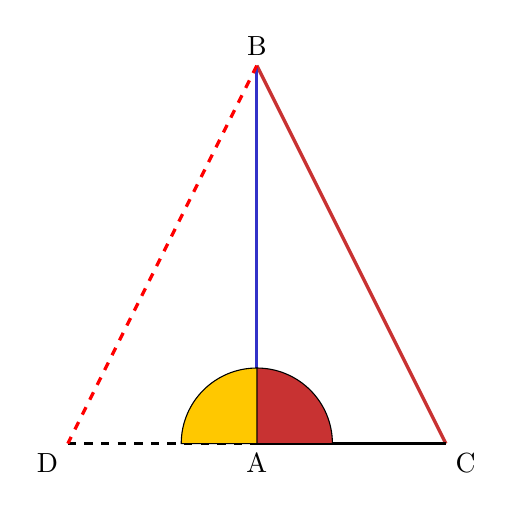
\begin{tikzpicture}[scale=1.2]
        \coordinate (A) at (0,0);
        \coordinate (B) at (0,4);
        \coordinate (C) at (2,0);
        \coordinate (D) at (-2,0);
        
        \draw[redsolid] (B) -- (C);
        \draw[bluesolid] (B) -- (A);
        \draw[blacksolid] (A) -- (C);
        \draw[blackdashed] (D) -- (A);
        \draw[reddashed] (B) -- (D);
        
        \draw[fill=redfig] (A) ++(0:0.8) arc (0:90:0.8) -- (A) -- cycle;
        \draw[fill=yellowfig] (A) ++(90:0.8) arc (90:180:0.8) -- (A) -- cycle;
        
        \node[above] at (B) {B};
        \node[below right] at (C) {C};
        \node[below] at (A) {A};
        \node[below left] at (D) {D};
        
    \end{tikzpicture}
\end{minipage}
\hfill
\begin{minipage}[t]{0.55\textwidth}
    \lettrine[lines=3, findent=2pt, nindent=0pt]Если в треугольнике квадрат одной стороны \redsegment{0.8} равен сумме квадратов двух других сторон \bluesegment{0.8} и \blacksegment{0.8}, то угол 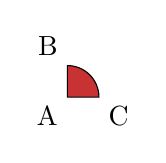
\begin{tikzpicture}[scale=0.4, baseline=(current bounding box.center)]
        \draw[fill=redfig] (0,0) -- (1,0) arc (0:90:1) -- cycle;
        \node[below left] at (0,0) {A};
        \node[above left] at (0,1) {B};
        \node[below right] at (1,0) {C};
    \end{tikzpicture}, заключенный между этими двумя сторонами прямой.
    
    \vspace{0.5cm}
    
    \begin{center}
        Проведем \blackdashedsegment{0.8} $\perp$ \bluesegment{0.8} \\
        и = \blacksegment{0.8} (пр. I.11, I.3) \\
        также проведем \redsegment{0.8}.
    \end{center}
    
    \vspace{0.3cm}
    
    \begin{center}
        Поскольку \blackdashedsegment{0.8} = \blacksegment{0.8} (постр.) \\
        \blackdashedsegment{0.8}$^2$ = \blacksegment{0.8}$^2$; \\
        
        $\therefore$ \blackdashedsegment{0.8}$^2$ + \bluesegment{0.8}$^2$ = \blacksegment{0.8}$^2$ + \bluesegment{0.8}$^2$ \\
        
        но \blackdashedsegment{0.8}$^2$ + \bluesegment{0.8}$^2$ = \reddashedsegment{0.8}$^2$ (пр. I.47), \\
        и \blacksegment{0.8}$^2$ + \bluesegment{0.8}$^2$ = \redsegment{0.8}$^2$ (гип.) \\
        
        $\therefore$ \reddashedsegment{0.8}$^2$ = \redsegment{0.8}$^2$, \\
        $\therefore$ \reddashedsegment{0.8} = \redsegment{0.8}; \\
        
        и $\therefore$ 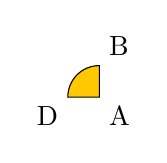
\begin{tikzpicture}[scale=0.4, baseline=(current bounding box.center)]
            \draw[fill=yellowfig] (0,0) -- (1,0) -- (1,1) arc (90:180:1) -- cycle;
            \node[below left] at (0,0) {D};
            \node[above right] at (1,1) {B};
            \node[below right] at (1,0) {A};
        \end{tikzpicture} = 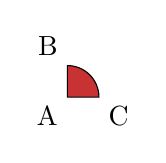
\begin{tikzpicture}[scale=0.4, baseline=(current bounding box.center)]
            \draw[fill=redfig] (0,0) -- (1,0) arc (0:90:1) -- cycle;
            \node[below left] at (0,0) {A};
            \node[above left] at (0,1) {B};
            \node[below right] at (1,0) {C};
        \end{tikzpicture} (пр. I.8), \\
        
        следовательно 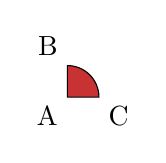
\begin{tikzpicture}[scale=0.4, baseline=(current bounding box.center)]
            \draw[fill=redfig] (0,0) -- (1,0) arc (0:90:1) -- cycle;
            \node[below left] at (0,0) {A};
            \node[above left] at (0,1) {B};
            \node[below right] at (1,0) {C};
        \end{tikzpicture} прямой угол.
    \end{center}
    
    \vspace{0.5cm}
    
    \begin{flushright}
    ч. т. д.
    \end{flushright}
\end{minipage}
\end{figure}

\end{document}